
\section{Inbetriebnahme eines OpenBTS Systems}
Für Inbetriebnahme des GSM Netzes waren einige Vorinstallationen sowie das Einrichten von Ubuntu 16.04.3 nötig. Im Folgenden wird das Vorgehen zur Einrichtung des Systems sowie die Inbetriebnahme des GSM Netzes beschrieben.

\subsection{Vorinstallationen}

\subsubsection{Ubuntu 16.04.3}
Zunächst wurde wie bei der Installation von Osmocom das Betriebssystem Ubuntu 16.04.3 auf einem Labor-Rechner installiert und eingerichtet. Zusätzlich wurden alle Programme und Pakete mit den folgenden Befehlen aktualisiert.
\begin{lstlisting}
sudo apt-get update
sudo apt-get upgrade
\end{lstlisting}

\subsubsection{Git}
Auch Range Networks nutzt für OpenBTS Git-Repositories, weshalb auch für die Installation von OpenBTS zunächst Git eingerichtet wurde. Zur Versionskontrolle und Verwaltung des Codes wurde auch hier das Team-interne Git Repository genutzt.
\begin{lstlisting}
sudo apt-get install software-properties-common python-software-properties
sudo add-apt-repository ppa:git-core/ppa
sudo apt-get update
sudo apt-get install git
\end{lstlisting}

\subsubsection{Softwarevoraussetzungen}
In vielen Installationsanleitungen werden zuerst eine Reihe von Bibliotheken und Paketen angegeben, die für die Installation von OpenBTS notwendig sein sollen. Range Networks hat die Installation dieser Pakete inzwischen ins Build-Skript integriert, sodass alle vorausgesetzten Abhängigkeiten später automatisch installiert werden sollten.

\subsubsection{Aktivierung der Verbindung zum USRP2}
Nachdem wir in Kapitel~\ref{usrp2_connect} die IP-Adresse des N210 erfolgreich zurücksetzen konnten, mussten wir in diesem Fall nur eine Verbindung zum USRP2-Gerät aufnehmen, indem wir die IP-Adresse des PCs innerhalb des gleichen Netzwerkbereichs setzten.
\begin{lstlisting}
sudo ifconfig enp0s25 192.168.10.3
\end{lstlisting}

Dieses mal konnten wir mithilfe der automatischen Erkennungsfunktion direkt erkennen, dass eine Verbindung zum N210 bestand.
\begin{lstlisting}
uhd_find_devices
\end{lstlisting}

Da uns im Laufe des Projekts die IP-Adresse der Schnittstelle am PC immer wieder zurückgesetzt wurde, speicherten wir die IP-Adresse daraufhin direkt in den Netzwerkeinstellungen.

\subsection{Installation}
Range Networks stellt eine detaillierte Anleitung zur Installation von OpenBTS inklusive aller zuvor beschriebenen Komponenten bereit, die zur Inbetriebnahme eines GSM-Netzes benötigt werden. Im Folgenden werden die Schritte zur Umsetzung auf der uns vorgelegenen Hardware genauer beschrieben.\\
\\
Die aktuellste Version von OpenBTS kann direkt aus dem Git-Repository von Range Networks geladen werden.
\begin{lstlisting}
sudo git clone https://github.com/RangeNetworks/dev.git
cd dev
sudo ./clone.sh
sudo ./switchto.sh master
\end{lstlisting}

Die Installation wird von Range Networks so leicht wie möglich gemacht, indem alle Komponenten zusammen aus ihren Git-Repositories heruntergeladen werden. Zugleich wird ein Build-Skript bereitgestellt, welches alle Build-Abhängigkeiten installiert und jede Komponente in ein installierbares Paket kompiliert.\\
Dafür muss lediglich das Build-Skript mit dem Namen des Transceivers als erstes Argument ausgeführt werden. Um einzelne Pakete zu kompilieren, kann zusätzlich optional der Name der Komponente als zweites Argument angegeben werden.
\begin{lstlisting}
#(vom OpenBTS root)
sudo ./build.sh N210 [component-name]
\end{lstlisting}

Dieser Schritt dauerte bei uns eine ganze Weile - geschätzt eine halbe Stunde. Im Anschluss sollten alle kompilierten Pakete im Unterverzeichnis BUILDS/<timestamp> zu finden sein. Die beiden Libraries \textit{libcoredumper} und \textit{liba53} werden auch gleichzeitig installiert, alle restlichen Software-Pakete müssen im folgenden Schritt manuell installiert werden.
\begin{lstlisting}
#(vom OpenBTS root)
sudo dpkg -i BUILDS/<timestamp>/*.deb
\end{lstlisting}

Um möglicherweise fehlende Abhängigkeiten aufzulösen, sollte noch folgender Befehl ausgeführt werden.
\begin{lstlisting}
sudo apt-get -f install
\end{lstlisting}

\subsection{Konfiguration}
Nachdem alle Komponenten erfolgreich installiert wurden, muss der für den USRP N210 passende Transceiver verlinkt werden.
\begin{lstlisting}
#(vom OpenBTS root)
cd apps
ln -s ../Transceiver52M/transceiver .
\end{lstlisting}

\subsubsection{Datenbanken initialisieren}
Nun mussten noch einige der Datenbanken erstellt werden. Für die Initialisierung stehen in den Programmverzeichnissen .sql-Dateien zur Verfügung. Zuerst haben wir den Ordner für die Datenbanken erstellt und dann die OpenBTS-Datenbank initialisiert.
\begin{lstlisting}
#(vom OpenBTS root)
sudo mkdir /etc/OpenBTS
sudo sqlite3 -init ./apps/OpenBTS.example.sql /etc/OpenBTS/OpenBTS.db ".quit"
\end{lstlisting}

Mit folgendem Befehl kann daraufhin getestet werden, ob die Datenbank erfolgreich initialisiert wurde. Wenn eine ganze Reihe an Zeilen ausgegeben werden - eine leere Datenbank dürfte nur drei Zeilen ausgeben - so scheint alles geklappt zu haben.
\begin{lstlisting}
sqlite3 /etc/OpenBTS/OpenBTS.db .dump
\end{lstlisting}

Die Datenbanken von SMQueue und SIPAuthServe wurden analog dazu initialisiert.
\begin{lstlisting}
#(vom OpenBTS root)
sudo sqlite3 -init subscriberRegistry/sipauthserve.example.sql /etc/OpenBTS/sipauthserve.db ".quit"
sudo sqlite3 -init smqueue/smqueue/smqueue.example.sql /etc/OpenBTS/smqueue.db ".quit"
\end{lstlisting}

Auch hier sollte getestet werden, ob die Datenbanken erfolgreich erstellt und mit Daten gefüllt wurden.
\begin{lstlisting}
sqlite3 /etc/OpenBTS/sipauthserve.db .dump
sqlite3 /etc/OpenBTS/smqueue.db .dump
\end{lstlisting}

\subsubsection{OpenBTS Einstellungen}
Um OpenBTS nun an unser Netz und die lizenzierten Frequenzen anzupassen, mussten wir hier einige Einstellungen vornehmen. Die Änderungen haben wir direkt in der OpenBTS.db Datenbank vorgenommen, welche wir mithilfe des Programms \textit{SQLitebrowser} geöffnet haben. Dieses mussten wir zunächst installieren und daraufhin starten.
\begin{lstlisting}
sudo apt-get install sqlitebrowser
sudo sqlitebrowser
\end{lstlisting}

Im Programm konnten wir dann die Datenbank unter /etc/OpenBTS/OpenBTS.db öffnen und so folgende Parameter anpassen.
\begin{table}[h]
	\centering
		\begin{tabular}{lll}
			\textbf{Control.LUR.OpenRegistration} & .* & // Registrierung für alle Teilnehmer erlauben\\
			\textbf{GSM.Identity.MCC} & 001 & // 001 für Testnetze\\
			\textbf{GSM.Identity.MNC} & 050 & // frei wählbar\\
			\textbf{GSM.Identity.ShortName} & mitm.de & // frei wählbar\\
			\textbf{GSM.Radio.Band} & 1900 & // GSM Frequenzband\\
			\textbf{GSM.Radio.C0} & 806 & // ARFCN des Frequenzbandes\\
			\textbf{GSM.Radio.RxGain} & 8 & // Empfängerverstärkung in dB.\\
			& & // Für Ettus Geräte zwischen 0-10 empfohlen.\\
		\end{tabular}
\end{table}

\begin{figure}[htbp]
	\centering
		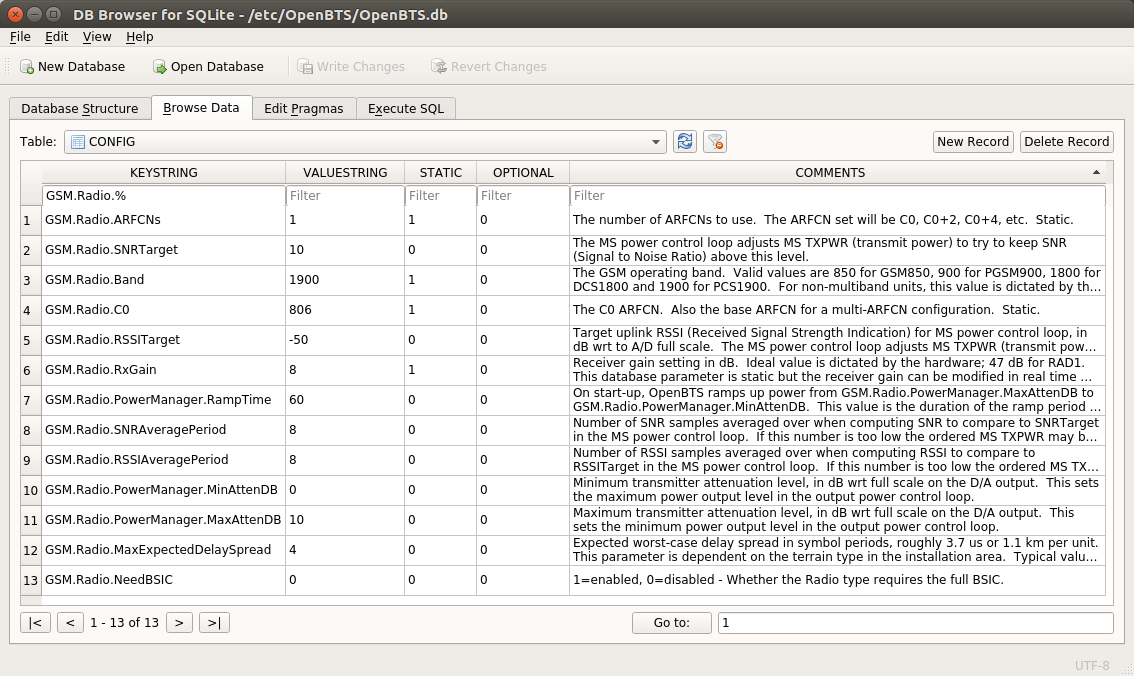
\includegraphics[width=1.0\textwidth]{includes/DB_OpenBts_GSMRadio}
	\caption{Ansicht in SQLitebrowser zur Konfiguration der OpenBTS.db-Datenbank}
	\label{fig:sqlitebrowser}
\end{figure}

Da wir OpenBTS zunächst ohne vorherige Anpassung der Einstellungen am Radioband gestartet haben, bekamen wir folgende Fehlermeldung nach dem Start des Transceivers. Diese verschwand als wir die entsprechenden Einstellungen gesetzt hatten.
\begin{lstlisting}
ALERT 2577:2596 2017-09-14T13:49:16.0 Transceiver.cpp:414:pullRadioVector: Clipping detected on RACH input
\end{lstlisting}

Da bei uns die Konfigurationsdateien von Asterisk nicht bei jeder Neuinstallation aktualisiert wurden, haben wir diese teilweise manuell zurückgesetzt.
\begin{lstlisting}
#(vom OpenBTS root)
sudo cp asterisk-config/* /etc/asterisk
\end{lstlisting}

Damit waren die Grundeinstellungen für den Betrieb von OpenBTS gesetzt.

\subsection{Starten des Systems}
Nach Installation aller Komponenten wurde das System gestartet. Die Reihenfolge spielt hierbei keine Rolle, da der Transceiver selbstständig von OpenBTS gestartet wird und alle Dienste über verschiedene Ports miteinander kommunizieren.\\
Um alle Programme später möglichst leicht starten zu können, wurden Links zu den ausführbaren Dateien im Userverzeichnis erstellt. Nur für OpenBTS wurde ein Link zum Überverzeichnis gesetzt, da das Starten ansonsten nicht funktionierte.
\begin{lstlisting}
#(vom Userverzeichnis)
sudo ln -s dev/asterisk/asterisk-11.7.0/main/asterisk .
sudo ln -s dev/smqueue/smqueue/smqueue .
sudo ln -s dev/subscriberRegistry/apps/sipauthserve
sudo ln -s dev/openbts/apps/
sudo mv apps openbts
\end{lstlisting}

So konnten die einzelnen Programme nun jederzeit ohne größere Suche der Dateien gestartet werden.
\begin{lstlisting}
#(vom Userverzeichnis)
sudo ./sipauthserve
sudo ./smqueue
sudo ./openbts/OpenBTS
sudo ./asterisk
\end{lstlisting}

Beim Start der verschiedenen Komponenten wurden uns folgende Zeilen ausgegeben.\\
\begin{figure}[htbp]
	\centering
		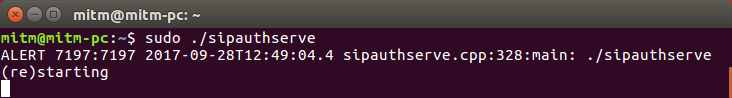
\includegraphics[width=0.90\textwidth]{includes/Start_sipauthserve}
	\caption{Ansicht der Konsole nach dem Start von SIPAuthServe}
	\label{fig:start_sipauthserve}
\end{figure}

\begin{figure}[htbp]
	\centering
		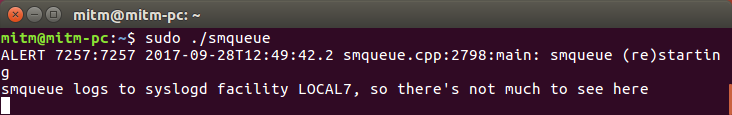
\includegraphics[width=0.90\textwidth]{includes/Start_smqueue}
	\caption{Ansicht der Konsole nach dem Start von SMQueue}
	\label{fig:start_smqueue}
\end{figure}

\begin{figure}[htbp]
	\centering
		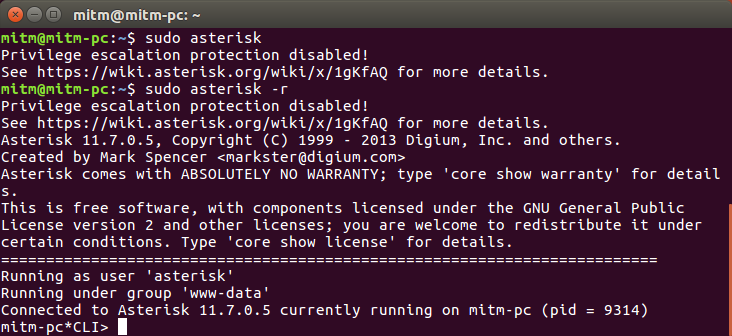
\includegraphics[width=0.90\textwidth]{includes/Start_asterisk}
	\caption{Ansicht der Konsole nach dem Start von Asterisk}
	\label{fig:start_asterisk}
\end{figure}

\newpage
\begin{figure}[htbp]
	\centering
		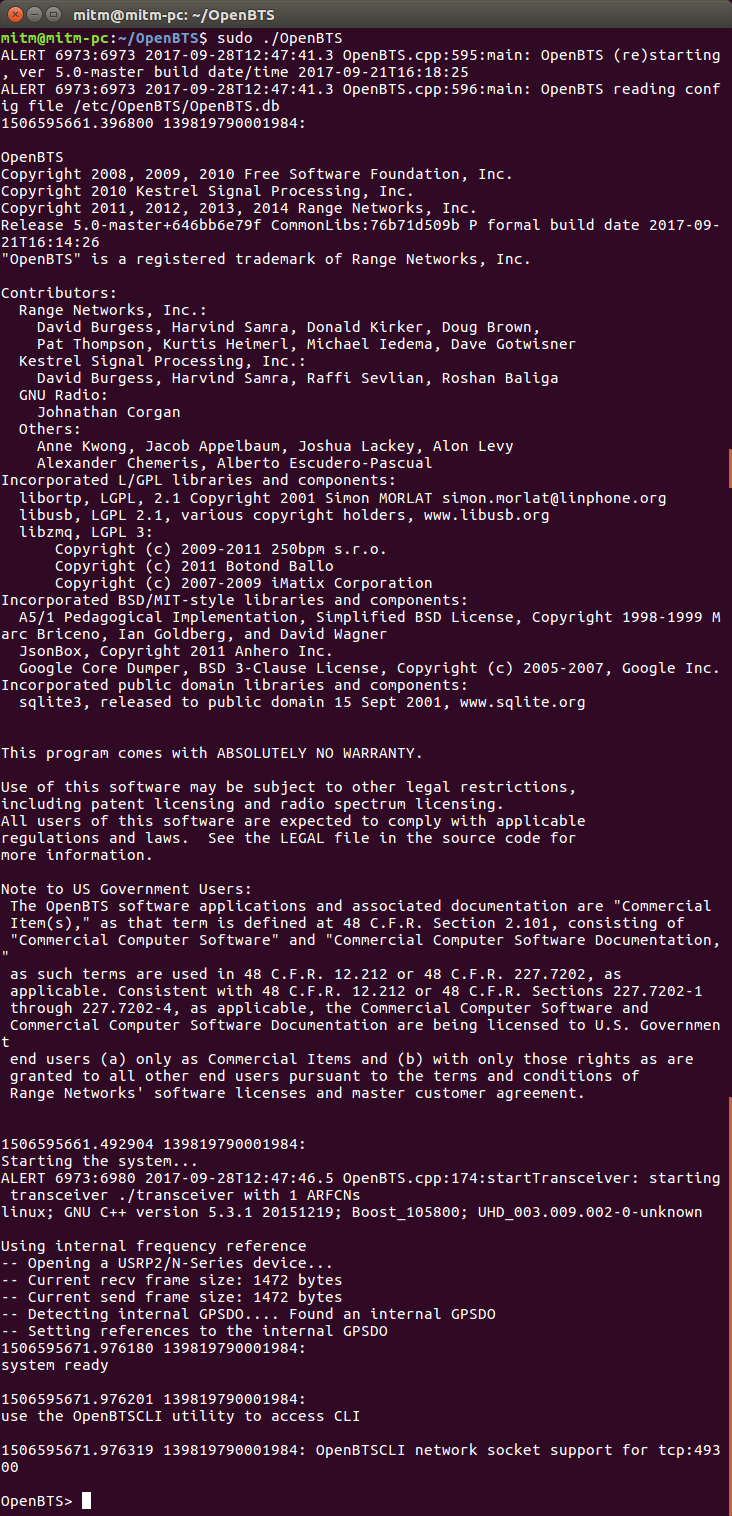
\includegraphics[width=0.70\textwidth]{includes/Start_OpenBTS}
	\caption{Ansicht der Konsole nach dem Start von OpenBTS}
	\label{fig:start_OpenBTS}
\end{figure}

\subsection{Testen der Funktionen}
Nach dem Start aller Anwendungen war es uns nun endlich möglich unser eigenes Mobilfunknetz zu testen. Natürlich funktionierte nicht alles sofort, vor allem die Asterisk-Einstellungen stellten uns vor einige Probleme. Letztendlich konnten alle elementaren Funktionen in Betrieb gesetzt werden, nachdem alle Einstellungen für eine ODBC-Verbindung zwischen Asterisk und der sqlite3.db Datenbank entfernt wurden. Diese ODBC-Schnittstelle sollte für eine Real-Time Verbindung sorgen, die sichere Verbindungen über Asterisk ermöglicht, da die Verbindungen ansonsten über externe Schnittstellen übertragen werden.\\
Nach erfolgreicher Anmeldung im Testnetz erhielten wir sofort eine Nachricht von der Nummer 101, die wir per Datenbank hätten anpassen können. Antwortet man nun mit einer 7-10 stelligen Nummer, so wird dem Endgerät diese Telefonnummer zugewiesen und in der sqlite3.db Datenbank unter der zugehörigen IMSI abgespeichert.

\begin{figure}[htbp]
	\centering
		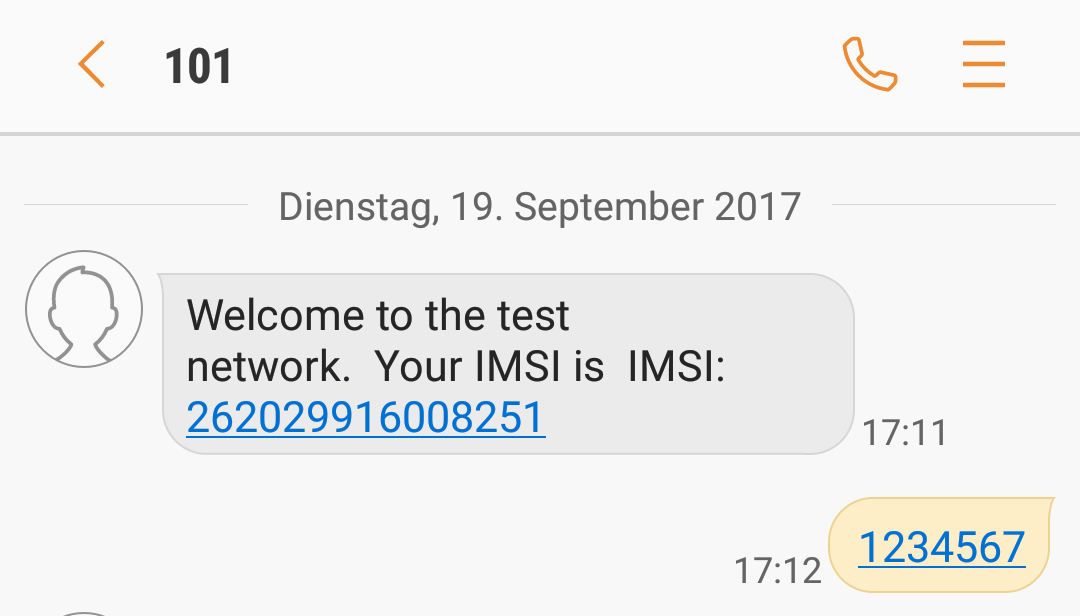
\includegraphics[width=0.6\textwidth]{includes/openbts_registration}
	\caption{Eingehende Nachricht nach erstmaliger Registrierung im Testnetz}
	\label{fig:openbts_registration}
\end{figure}

\begin{figure}[htbp]
	\centering
		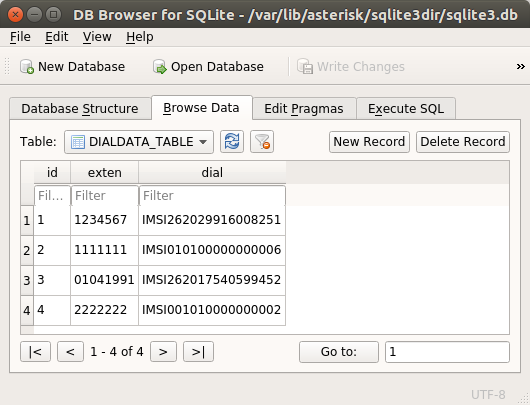
\includegraphics[width=0.9\textwidth]{includes/DB_asterisk_dialtable}
	\caption{Tabelle DIALTABLE in sqlite3.db nach Registrierung mehrerer Endgeräte}
	\label{fig:asterisk_dialtable}
\end{figure}

\begin{figure}[htbp]
	\centering
		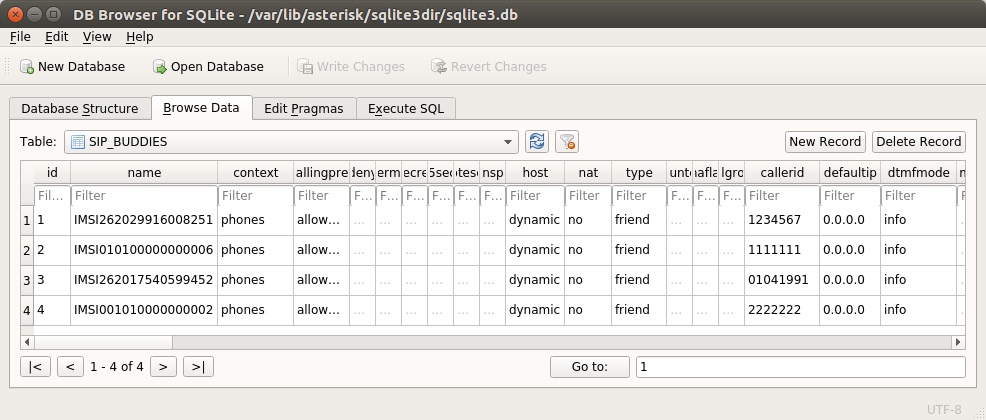
\includegraphics[width=0.9\textwidth]{includes/DB_asterisk_SipBuddies}
	\caption{Tabelle SIP\_BUDDIES in sqlite3.db nach Registrierung mehrerer Endgeräte}
	\label{fig:asterisk_sipbuddies}
\end{figure}

Das Senden von Nachrichten an verschiedene Teilnehmer im Netzwerk funktionierte schon von Beginn an einwandfrei. Nachdem wir die richtigen Einstellungen für Asterisk gefunden hatten, funktionierten sowohl Anrufe zu Testnummern, als auch zwischen den Teilnehmern. In Asterisk wurde nach einem Anruf eine Nachricht ausgegeben, die folgendermaßen aussah.

\begin{figure}[htbp]
	\centering
		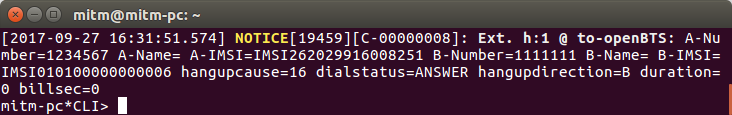
\includegraphics[width=0.9\textwidth]{includes/asterisk_call}
	\caption{Ausgabe in Asterisk nach Beenden eines Anrufs zwischen Mobilfunkteilnehmern}
	\label{fig:asterisk_call}
\end{figure}

\newpage